% \documentclass[portrait,25pt]{sciposter}
\documentclass[]{beamer}
\usepackage[orientation=portrait,size=a0extended,scale=1,debug]{beamerposter}
\usepackage[utf8x]{inputenc}
\usepackage[spanish]{babel}
\usepackage{amsmath}
\usepackage{amsfonts}
\usepackage{amssymb}
\usepackage{wasysym}
\usepackage{graphicx}
\usepackage{eurosym}
\usepackage{multicol}
\usepackage{fancyhdr}
\usepackage{tikz}
\usepackage{colortbl}
\usepackage[version=3]{mhchem}
\usepackage[lf]{venturis}

\setbeamertemplate{caption}[numbered] 

%\event{VII Congreso de Investigadores en Formaci\'on -- Universidad de C\'ordoba}
\date{VII Congreso de Investigadores en Formaci\'on\\ 
Universidad de C\'ordoba (6 y 7 de Febrero de 2019)}
\title{Demograf\'ia y Pensiones. Recursos de Planificaci\'on Financiera a Largo Plazo: La Hipoteca Inversa como Complemento a la Pensi\'on}
\author{Jos\'e Rafael Caro Barrera}
\institute{Dir.: Dr. D. Jos\'e M\textsuperscript{a} Caridad y Ocer\'in - Dpto. de Estad\'istica, Econometr\'ia e Investigaci\'on Operativa}


%%%%%%%%%%%%%%%%%%%%
% Document started %
%%%%%%%%%%%%%%%%%%%%

\mode<presentation>{
\usetheme{Regensburg}
\usecolortheme{PhysikPoster}
}

\begin{document}
\begin{frame}{\vspace{1ex}\hfill Palabras clave: \bfseries \textit{Demograf\'ia, Longevidad, Mortalidad, Pensiones, Planificaci\'on Financiera, Jubilaci\'on, Hipoteca Inversa.}}
	\begin{columns}[t]
	\column{.45\columnwidth}

\vspace{-1.5cm}
%%%%%%%%%%%%%%%% RESUMEN (ABSTRACT)%%%%%%%%%%%%%%%%%
\begin{block}{Resumen}
			
			\small
			\begin{multicols}{2}
				\setbeamertemplate{bibliography item}[text]
				\bibliographystyle{unsrt}
				\bibliography{literature}
				Se pone de relieve la situaci\'on demogr\'afica actual a todos los niveles, m\'as concretamente, se estudia el sistema de pensiones espa\~nol y se destaca la insuficiencia de los recursos p\'ublicos para garantizar las prestaciones sociales de la vejez, proponi\'endose alternativas de ahorro y liquidez como complemento a la pensi\'on.
			\end{multicols}
		\end{block}
		
		\vspace{-0.5cm}  %%%%%%%%%%%%%%%%%%%%%%%%%%%%%%%%%%%%%%%%%%%%%%%	
		\begin{block}{Estructura y Metodolog\'ia}
			\setlength{\parindent}{1.2em}
			\setlength{\parskip}{0.5ex}
			En una primera parte (que consta de 5 cap\'itulos) se tratan aspectos te\'oricos sobre demograf\'ia, modelos de predicci\'on de la mortalidad y pensiones. En la segunda parte, de 2 cap\'itulos, se abordan aspectos pr\'acticos sobre planificaci\'on financiera y se exponen las conclusiones m\'as relevantes. 
		\end{block}
		
\vspace{-0.5cm}

		\begin{block}{Los Fen\'omenos Demogr\'aficos}
			\begin{multicols}{2}
				\setlength{\parindent}{1.2em}
				\setlength{\parskip}{1ex}

				El mundo envejece. Y lo hace porque est\'a sufriendo una transformaci\'on demogr\'afica. El ser humano vive m\'as tiempo, la esperanza de vida se ha incrementado y las tasas de fertilidad est\'an decreciendo (ver figuras \ref{esperanza} y \ref{fertilidad}). As\'i:

				\begin{itemize}
					\item I) se espera que la esperanza de vida global sea de 83 a\~nos en 2095 y
					\item II) que la tasa de fertilidad disminuya hasta los dos nacimientos por mujer.
					%\item C
				\end{itemize}
				\vspace{-0.3cm}
				\begin{figure}[h]
					\centering
					\fbox{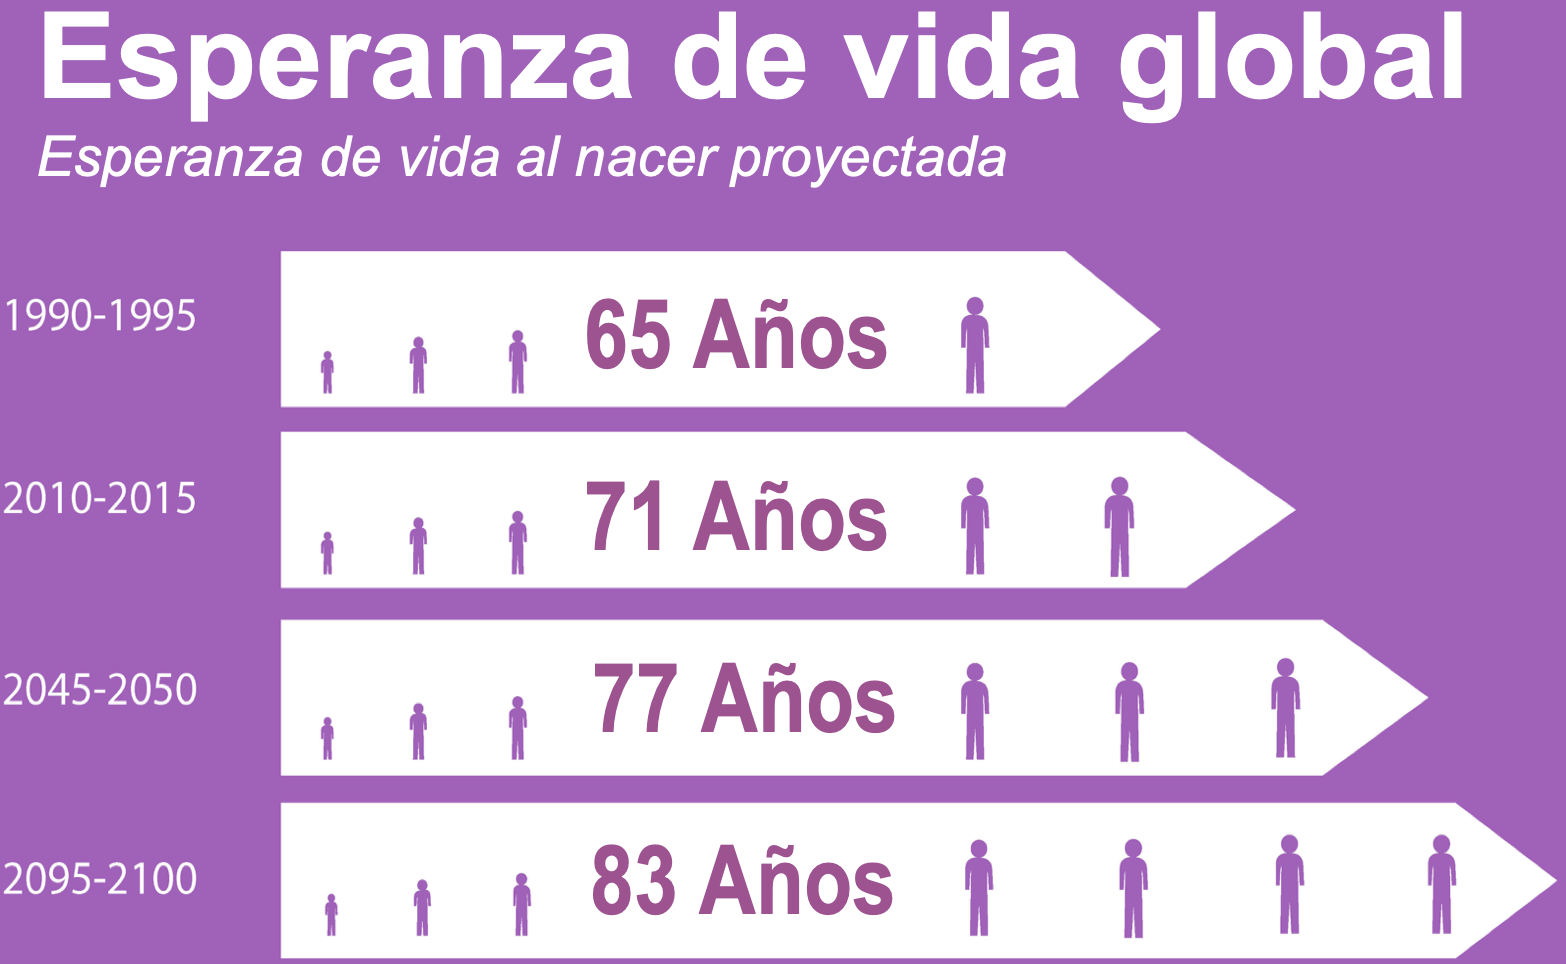
\includegraphics[width=.9\columnwidth]{esperanza.png}}
					\caption{\small Fuente: \textit{World Population Prospects: The 2017 Revision.}}
					\label{esperanza}
				\end{figure}

				\begin{figure}[h]
					\centering
					\fbox{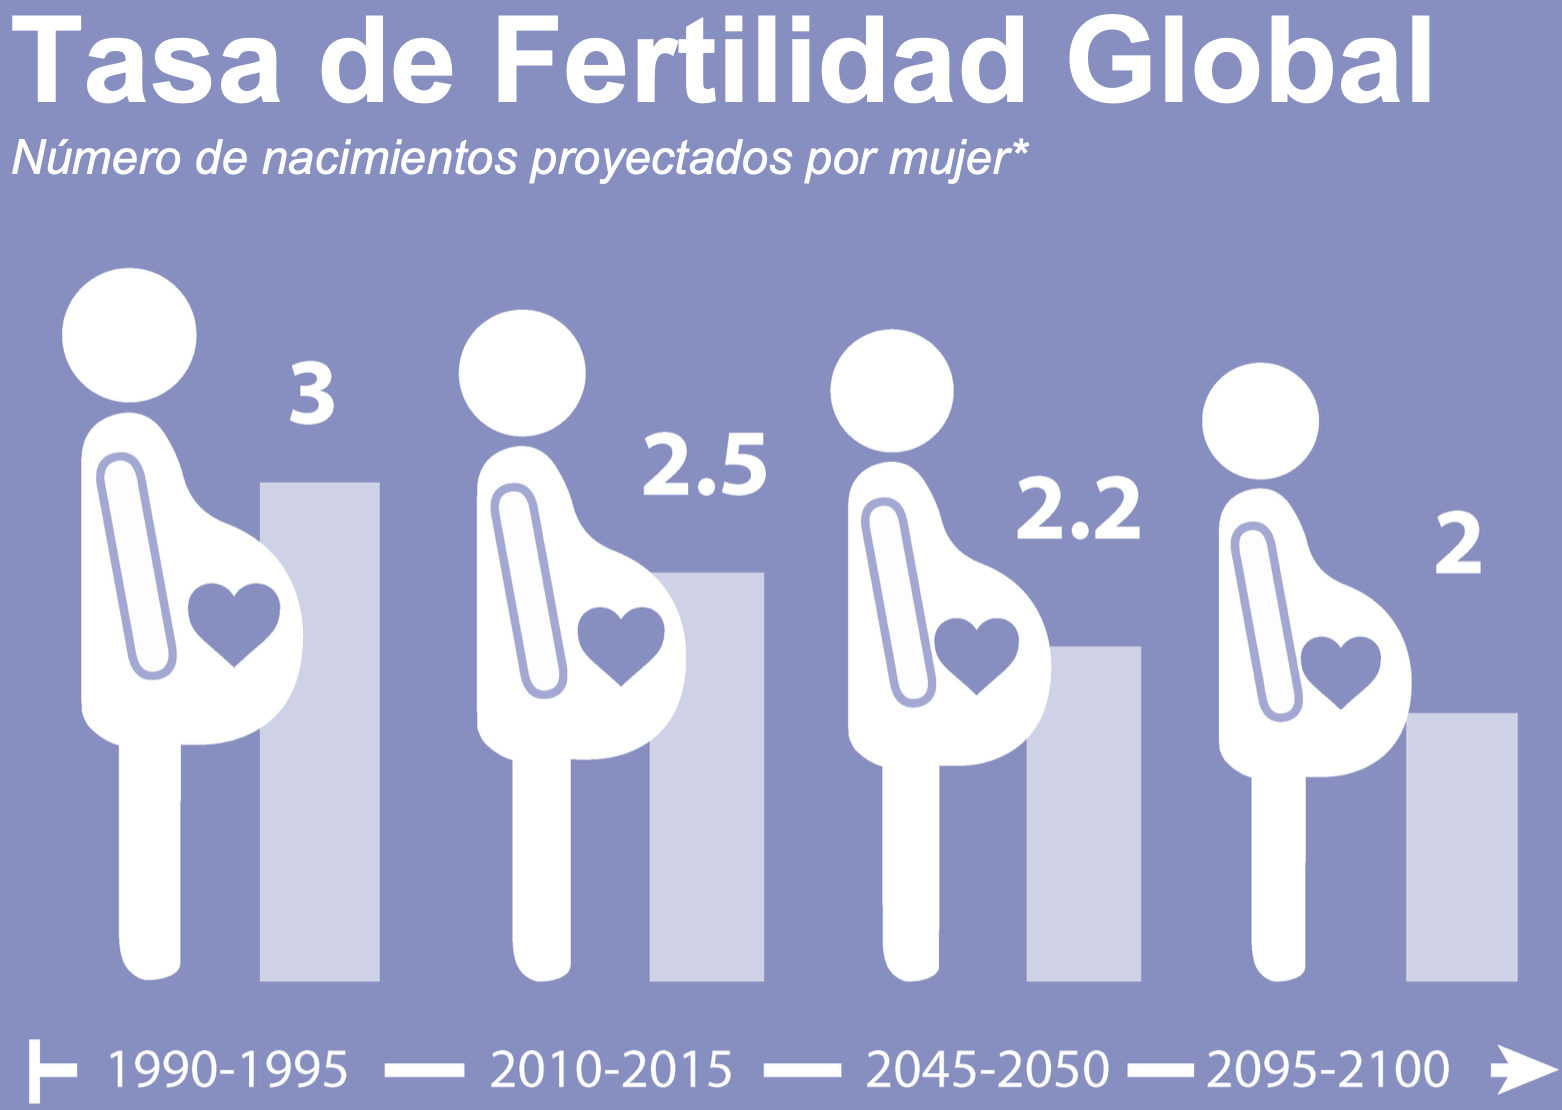
\includegraphics[width=.9\columnwidth]{fertilidad.png}}
					\caption{\small Fuente: \textit{World Population Prospects: The 2017 Revision.}  Dept. de Econom\'ia y Asuntos Sociales de las Naciones Unidas.}
					\label{fertilidad}
				\end{figure}
				\begin{figure}[h]
					\centering
					\fbox{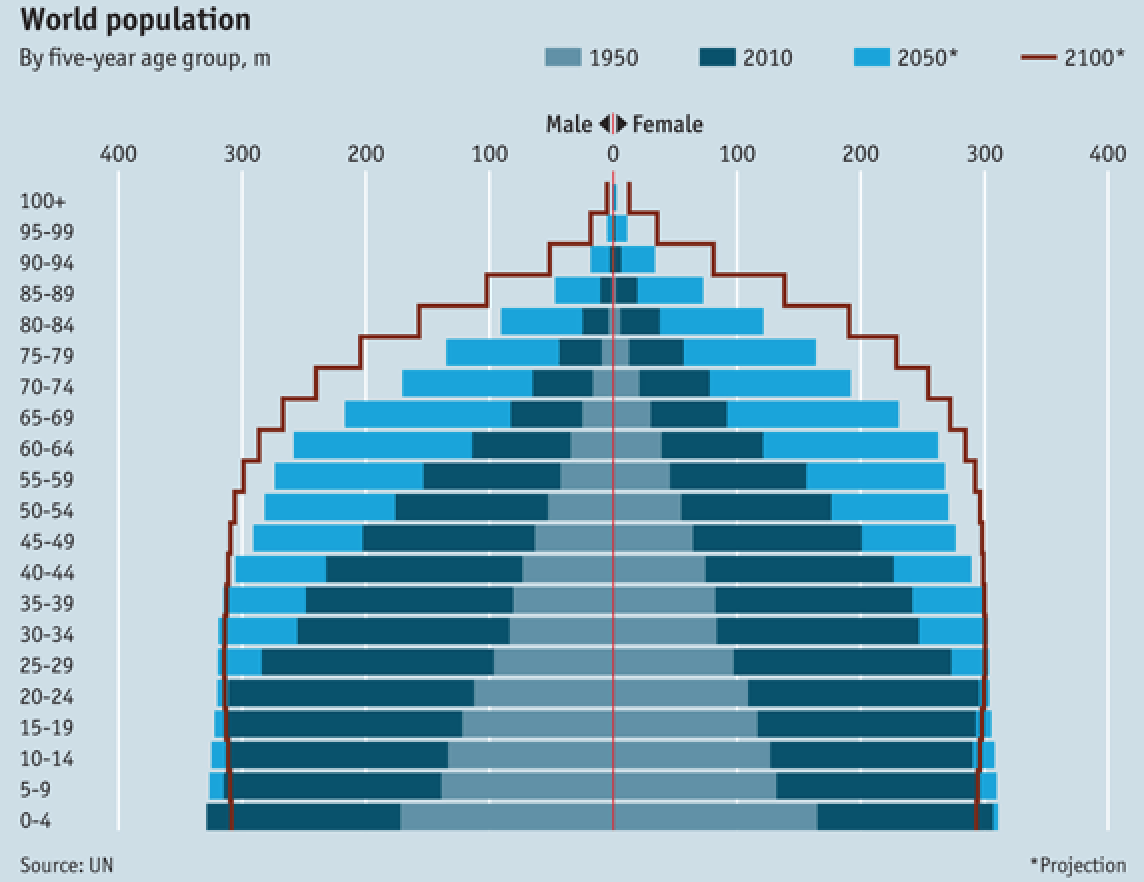
\includegraphics[width=.89\columnwidth]{piramide.png}}
					\caption{\small Estructura de la poblaci\'on mundial. Fuente: \textit{ONU.}}
					\label{piramide}
					\end{figure}
					\vspace{-0.4cm}
				La evoluci\'on de la estructura de edad de la poblaci\'on permite comprender mejor el envejecimiento. La figura \ref{piramide} muestra la evoluci\'on de la poblaci\'on mundial y la proyecci\'on para 2100.
				%Lorem ipsum dolor sit amet, consectetur adipiscing elit, sed do eiusmod tempor incididunt ut labore et dolore magna aliqua. Ut enim ad minim veniam, quis nostrud exercitation ullamco laboris nisi ut aliquip ex ea commodo consequat. Duis aute irure dolor in reprehenderit in voluptate velit esse cillum dolore eu fugiat nulla pariatur. 
				\begin{figure}[h]
					\centering
					\fbox{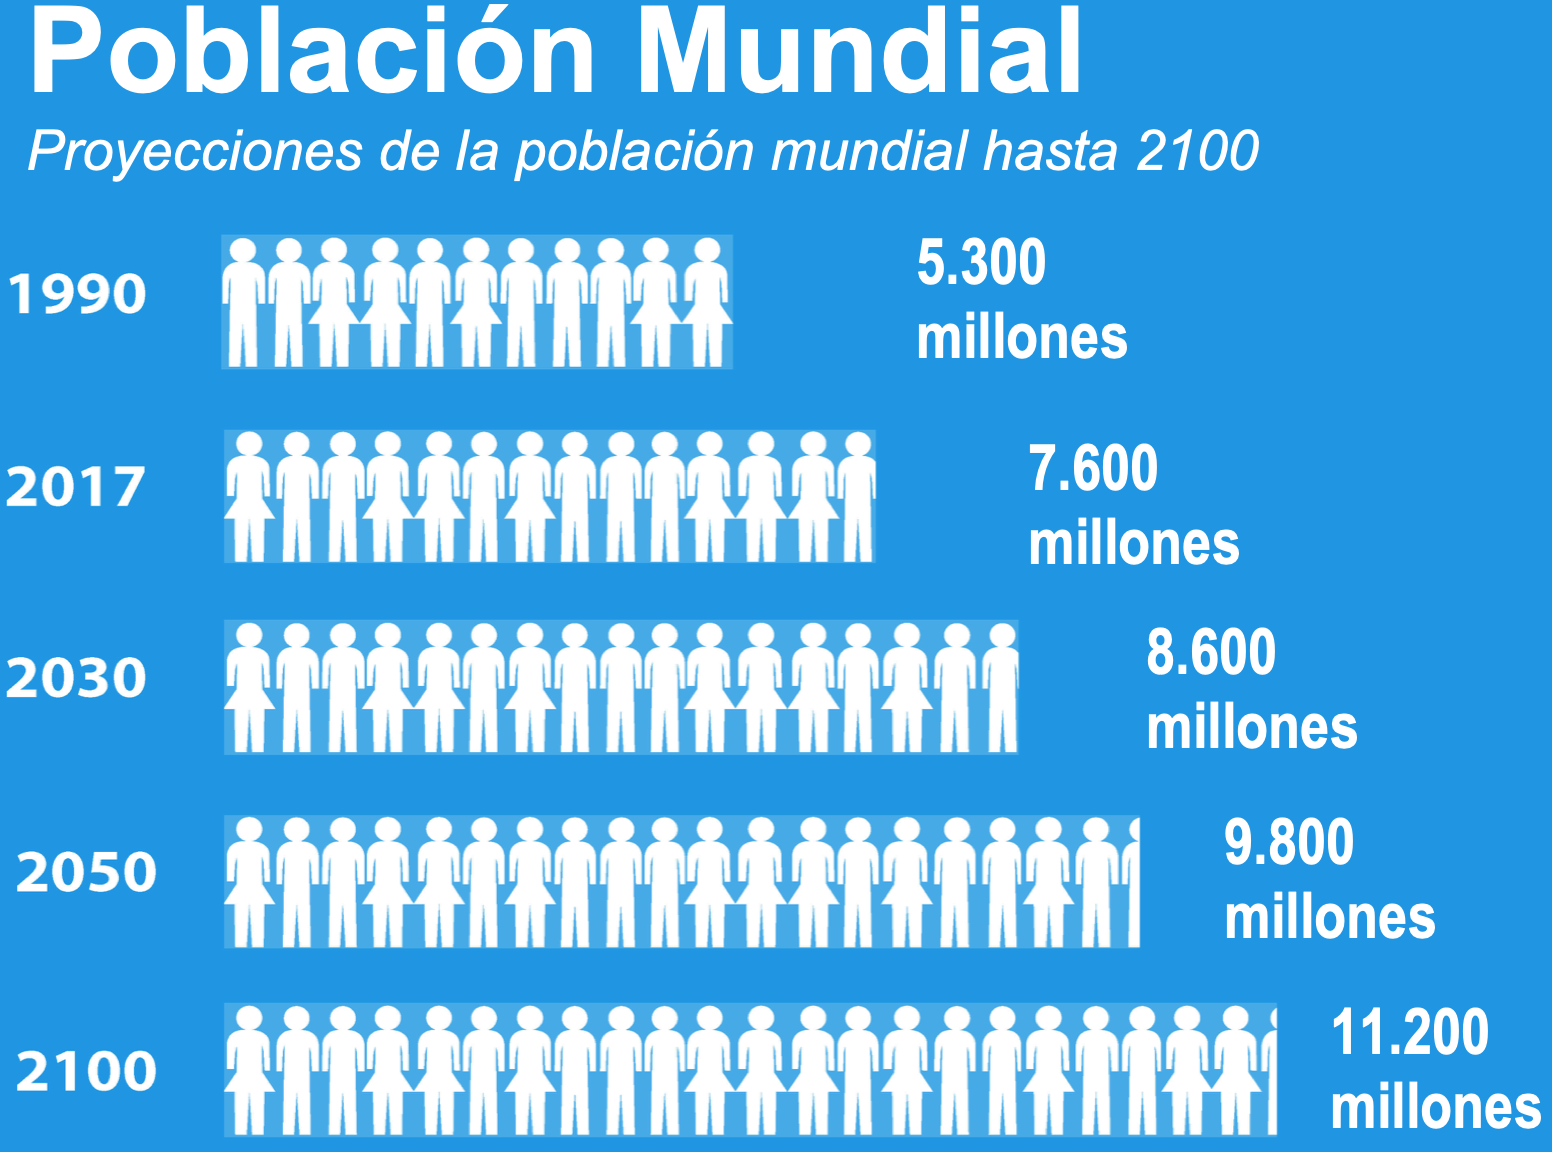
\includegraphics[width=.9\columnwidth]{poblacion.png}}
					\caption{\small Fuente: \textit{World Population Prospects: The 2017 Revision.}  Dept. de Econom\'ia y Asuntos Sociales de las Naciones Unidas. }
					\label{poblacion}
				\end{figure}
				\vspace{-0.9cm}
				Se prev\'e un incremento del 47\% de la poblaci\'on mundial en los pr\'oximos 80 a\~nos.
				%Lorem ipsum dolor sit amet, consectetur adipiscing elit, sed do eiusmod tempor incididunt ut labore et dolore magna aliqua.
			\end{multicols}
		\end{block}

\vspace{-0.5cm}
%%%%%%%%%%%%%%%%%%% MODELOS DE MORTALIDAD  %%%%%%%%%%%%%%%%%%%%
		\begin{block}{Modelos Estoc\'asticos de Mortalidad}\vspace{-0.5cm}
			\setlength{\parindent}{1.2em}
			\setlength{\parskip}{1ex}

			A medida que la esperanza de vida crece, el desarrollo futuro de la misma es incierto, es lo que se conoce como \textbf{riesgo de longevidad}. Esto conlleva un riesgo sistem\'atico para los planes de pensi\'on.
			%Lorem ipsum dolor sit amet, consectetur adipiscing elit, sed do eiusmod tempor incididunt ut labore et dolore magna aliqua. Ut enim ad minim veniam, quis nostrud exercitation ullamco laboris.
\vspace{-1cm}     %%%%%%%%%%%%%%% CARACTERÍSTICAS  %%%%%%%%%%%%%%%%%%%

			\begin{columns}[t]
				\column{.45\columnwidth}
				\begin{block}{Necesidad de los modelos}
					\begin{itemize}
						\item Con datos fiables, el proceso subyacente de estos datos es conducido por un proceso estoc\'astico.
						\item Incertidumbre de la evoluci\'on de la mortalidad.
						\item Permiten una adecuada \textbf{gesti\'on del riesgo de longevidad}.
						\item Establecen reservas de riesgo.
						\item Permiten dise\~nar \textit{contratos de seguros de vida con opciones integradas.}
						\item Fijaci\'on de precios y cobertura de valores vinculados a la mortalidad.													%\begin{itemize}
						%	\item Quis autem vel eum iure reprehenderit qui in ea.
						%\end{itemize}
						%\begin{itemize}
							%\item Lor separat existentie es un myth. 
						%\end{itemize}
					\end{itemize}
				\end{block}
				\column{.45\columnwidth} %%%%%%%%%% MODELOS MÁS IMPORTANTES  %%%%%%%
				\begin{block}{Modelos m\'as importantes}
				\vspace{-0.4cm}
				\textit{Lee-Carter}, (1992); \textit{Renshaw-Haberman}, (2006); \textit{Age-Period-Cohort} (APC); \textit{Cairns-Blake-Dowd}, (2006); \textit{Cairns y otros}, (2007a y 2007b),...
				\end{block}\vspace{-1cm}
				\begin{block}{Comparaci\'on de estos modelos}
				\setlength{\parindent}{1.2em}
				\setlength{\parskip}{1ex}\vspace{-1cm}
					\noindent Conforme a dos criterios:\vspace{-0.3cm} 
					\begin{enumerate}
						\item Criterio Cuantitativo:
						\begin{enumerate}
							\item[$\Rightarrow$] Criterio de Informaci\'on de Bayes (BIC).
							\item[$\Rightarrow$] Incompleto. No proporciona toda la informaci\'on.
						\end{enumerate}
						\item Criterio Cualitativo;
						\begin{enumerate}
							\item[$\Rightarrow$] Sensatez y transparencia.
							\item[$\Rightarrow$] Robustez relativa a la edad y al periodo.
							\item[$\Rightarrow$] Biol\'ogicamente razonable.
							\item[$\Rightarrow$] Predicciones razonables.					
						\end{enumerate}
						%\item Maecenas tempus spectrae.
						%\item Quisque rutrum. Aenean imperdiet.
					\end{enumerate}

					%~ \begin{flushright}
						%~ \includegraphics[height=10ex]{python_logo}
						%~ \includegraphics[height=10ex]{scipy_logo}
					%~ \end{flushright}

				\end{block}
			\end{columns}
			
			\vspace{-0.6cm}
			\begin{figure}[h]
				\centering
				%\begin{columns}[t]
				%\column{.33\columnwidth}
				     %\fbox{\includegraphics[width=.88\columnwidth]{modelos.png}}
					\fbox{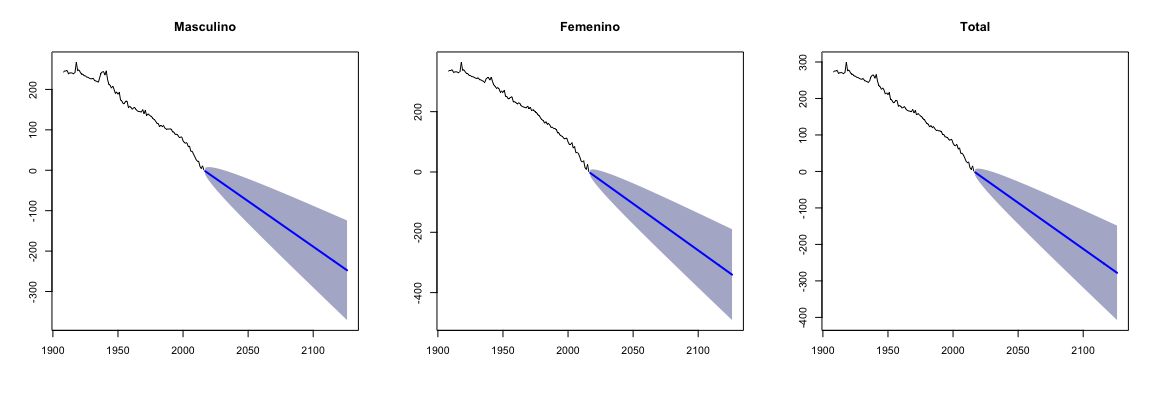
\includegraphics[width=.99\columnwidth]{mortesp4.png}}
					\caption{\small  Aplicaci\'on de la versi\'on original del modelo Lee-Carter para a obtener la predicci\'on de las tasas de mortalidad mediante el uso del paquete \textbf{`forecast'} en \textttt{\textbf{R}} y proyectar la tasa $k_{t}$ futura (tendencia temporal subyacente, hasta 110). La proyecci\'on est\'a basada en una extrapolaci\'on ARIMA. Se aprecia el patr\'on pasado y la predicci\'on futura de la tasa, seg\'un la poblaci\'on, para personas de 65 a\~nos.}
					%\caption{\small Gr\'aficos de dispersi\'on para las tasas de mortalidad $qxt$ en las edades $x = 65$ (abanico inferior), $x = 75$ (abanico medio) y $x = 85$ (abanico superior) de tres modelos ajustados a la poblaci\'on masculina de Inglaterra y Gales para las edades de 55-89 y per\'iodo 1961-2011. Los puntos muestran tasas hist\'oricas de mortalidad para 1961-2011. Las sombras en el abanico representan los intervalos de predicci\'on al 50\%, 80\% y 95\%.}
					\label{modelos}
				%\column{.32\columnwidth}
				%	\includegraphics[width=0.9\columnwidth]{gr\'afico_2.png}
				%	\caption{\small }
				%	\label{fig_background-removal}
				%\column{.32\columnwidth}
				%	\includegraphics[width=0.9\columnwidth]{gr\'afico_3.png}
				%	\caption{\small }
				%	\label{fig_energy-calibration}
			%	\end{columns}
			\end{figure}
\vspace{-0.2cm} %-0.5cm en la otra versión
			%Lorem ipsum dolor sit amet, consectetur adipiscing elit, sed do eiusmod tempor incididunt ut labore.
		\end{block}
%\vspace{-0.5cm}  %%%%%%%%%%%%%%%%%%%%%%%%%%%%%%%%%%%%%%%%%%%%%%%	
%		\begin{block}{ABCEFDAGADFA}
%			\setlength{\parindent}{1.2em}
%			\setlength{\parskip}{1ex}

%			Using the Python programming language we have written a program (licensed under GPL, available for download at \cite{emcd_tool}) for the comfortable treatment of EELS spectra for determination of EMCD signals.
%		\end{block}
%%%%%%%%%%%%%%%%%%%%%%%%%%%%%%%%%%%%%%%%%%%%%%%	
	
	\column{.515\textwidth}\vspace{-1.5cm}   %%%%%%% LAS PENSIONES EN ESPAÑA %%%%%%%%%%%
		
		\begin{block}{Las Pensiones en Espa\~na: Planificaci\'on Financiera de la Jubilaci\'on}
					\begin{figure}[h]
						\fbox{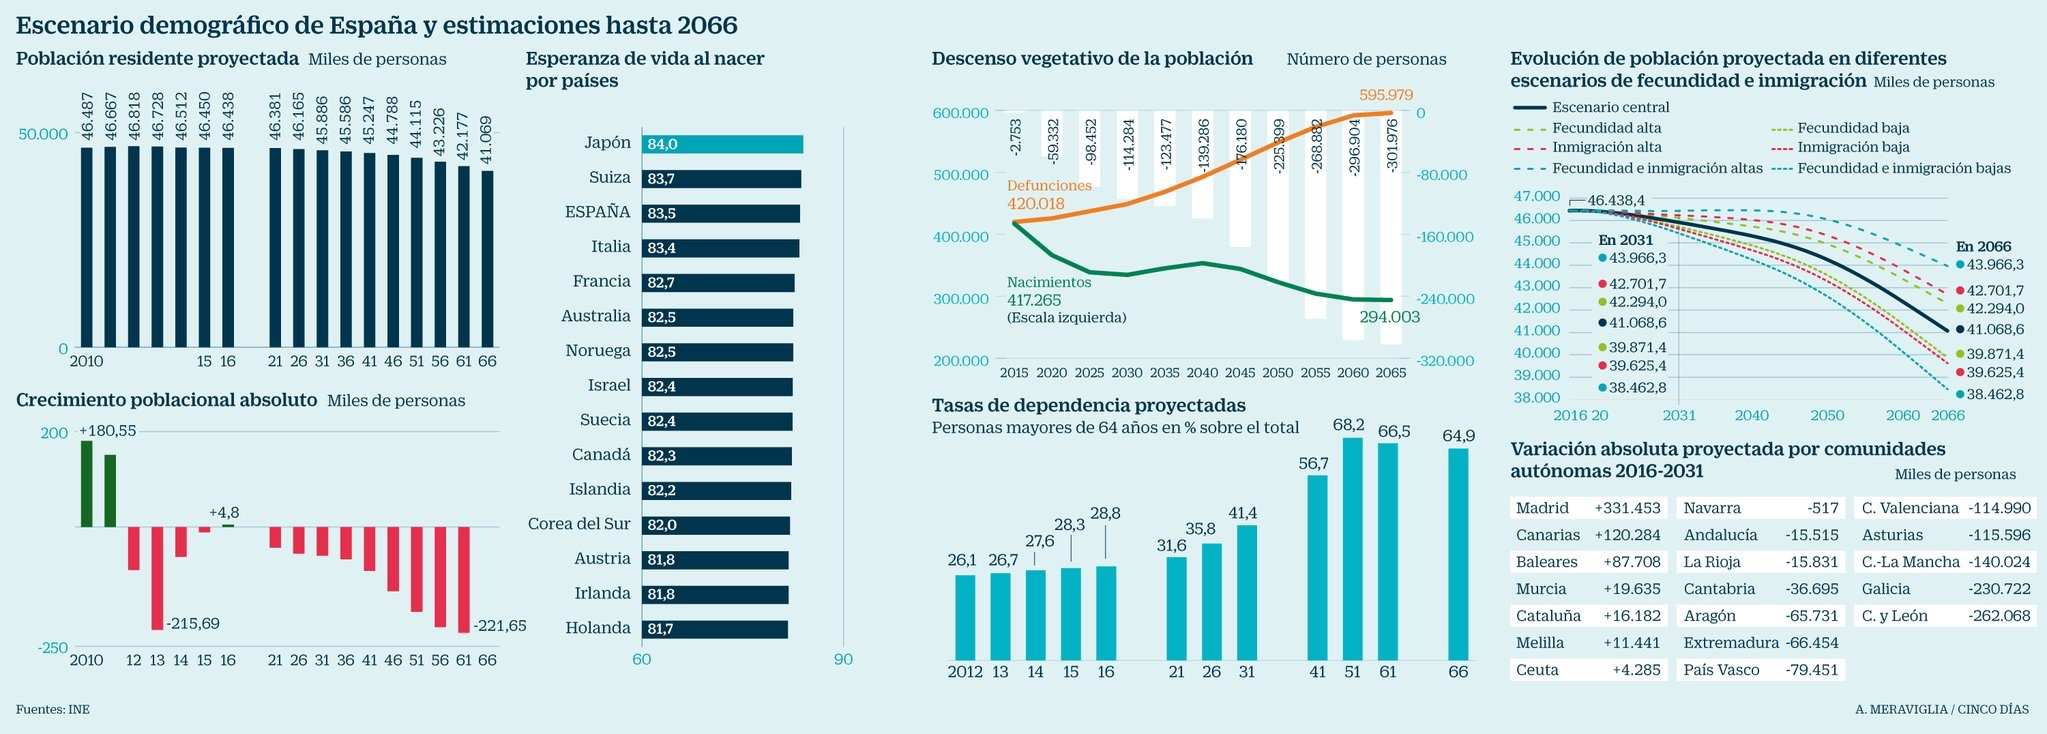
\includegraphics[width=.99\columnwidth]{pension1.jpg}}
						\caption{\small Radiograf\'ia del sistema de pensiones espa\~nol. Escenario demogr\'afico y estimaciones hasta 2066. \textit{Fuente: INE.}}
						\label{pension1}
					\end{figure}\vspace{-1cm}
			%\begin{columns}[t]
				%\column{.45\columnwidth}
					%\begin{figure}[h]
						%\includegraphics[width=.6\columnwidth]{gr\'afico_4.png}
						%\caption{\small Lorem ipsum dolor sit amet, consectetuer adipiscing elit. Aenean commodo ligula eget dolor. Aenean massa. Cum sociis natoque penatibus et magnis dis parturient montes.}
						%\label{emcd_twinview}
					%\end{figure}
				%\column{.45\columnwidth}
					%\begin{figure}[h]
						%\includegraphics[width=.6\columnwidth]{gr\'afico_5.png}
						%\caption{\small Lorem ipsum dolor sit amet, consectetuer adipiscing elit. Aenean 								commodo ligula eget dolor. Aenean massa.}
						%\label{emcd_70}
					%\end{figure}
			%\end{columns}
			\begin{multicols}{2}
					\begin{itemize}
						\item El gasto en pensiones aument\'o un 7\% en enero, hasta la cifra de 9.535 millones de \euro.
						\item Los efectos del envejecimiento deben contrarrestarse mediante un conjunto amplio de pol\'iticas: natalidad, conciliaci\'on, inmigraci\'on, reformas estructurales,...
						\item En Espa\~na, las condiciones demogr\'aficas del pasado y favorables para el sistema, no se repetir\'an en el futuro, por lo que se debe asegurar la sostenibilidad del mismo.
						\item En nuestro pa\'is, el importe medio de la pensi\'on es de 938 \euro\ y de la pensi\'on de jubilaci\'on de 1.085 \euro.						
						%\item Application of a filter reduces noise considerably, \textbf{but} gives rise to "background oscillations" (see fig. \ref{emcd_70}).
						%\item Increasing the kernel size of the filter results in stronger reduction of noise, \textbf{but} broadens features and decreases the height of the \ce{L23} edges.
					\end{itemize}
			\end{multicols}
			\vspace{-2.5cm}
			\begin{columns}[t]
				\column{.48\columnwidth}
					\begin{figure}[h]
						\fbox{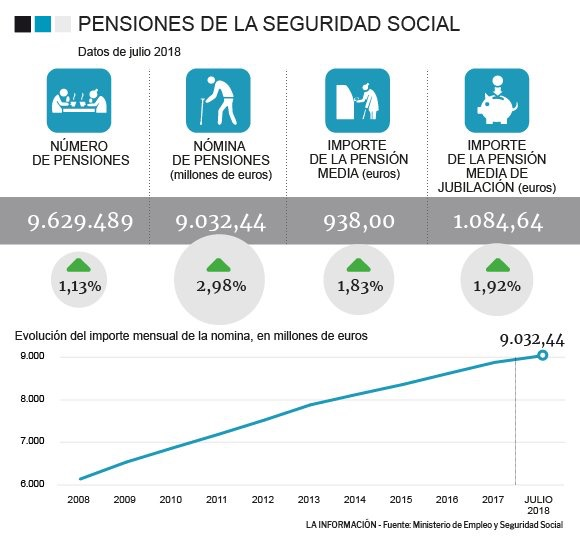
\includegraphics[width=\columnwidth]{pension2.jpg}}
						\caption{\small Fuente: Ministerio de Empleo y Seguridad Social.}
						\label{pension2}
					\end{figure}\vspace{-2cm}
					\begin{figure}[h]
						\fbox{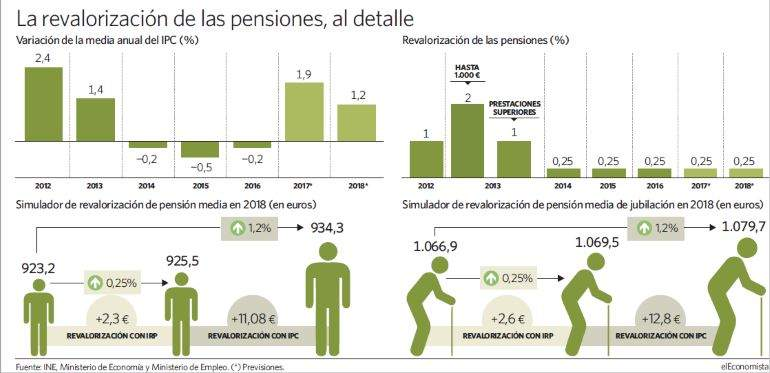
\includegraphics[width=\columnwidth]{reval.jpg}}
						\caption{\small Fuente: Ministerio de Empleo y Seguridad Social.}
						\label{reval}
					\end{figure}
				\column{.48\columnwidth}
					\begin{figure}[h]
						\fbox{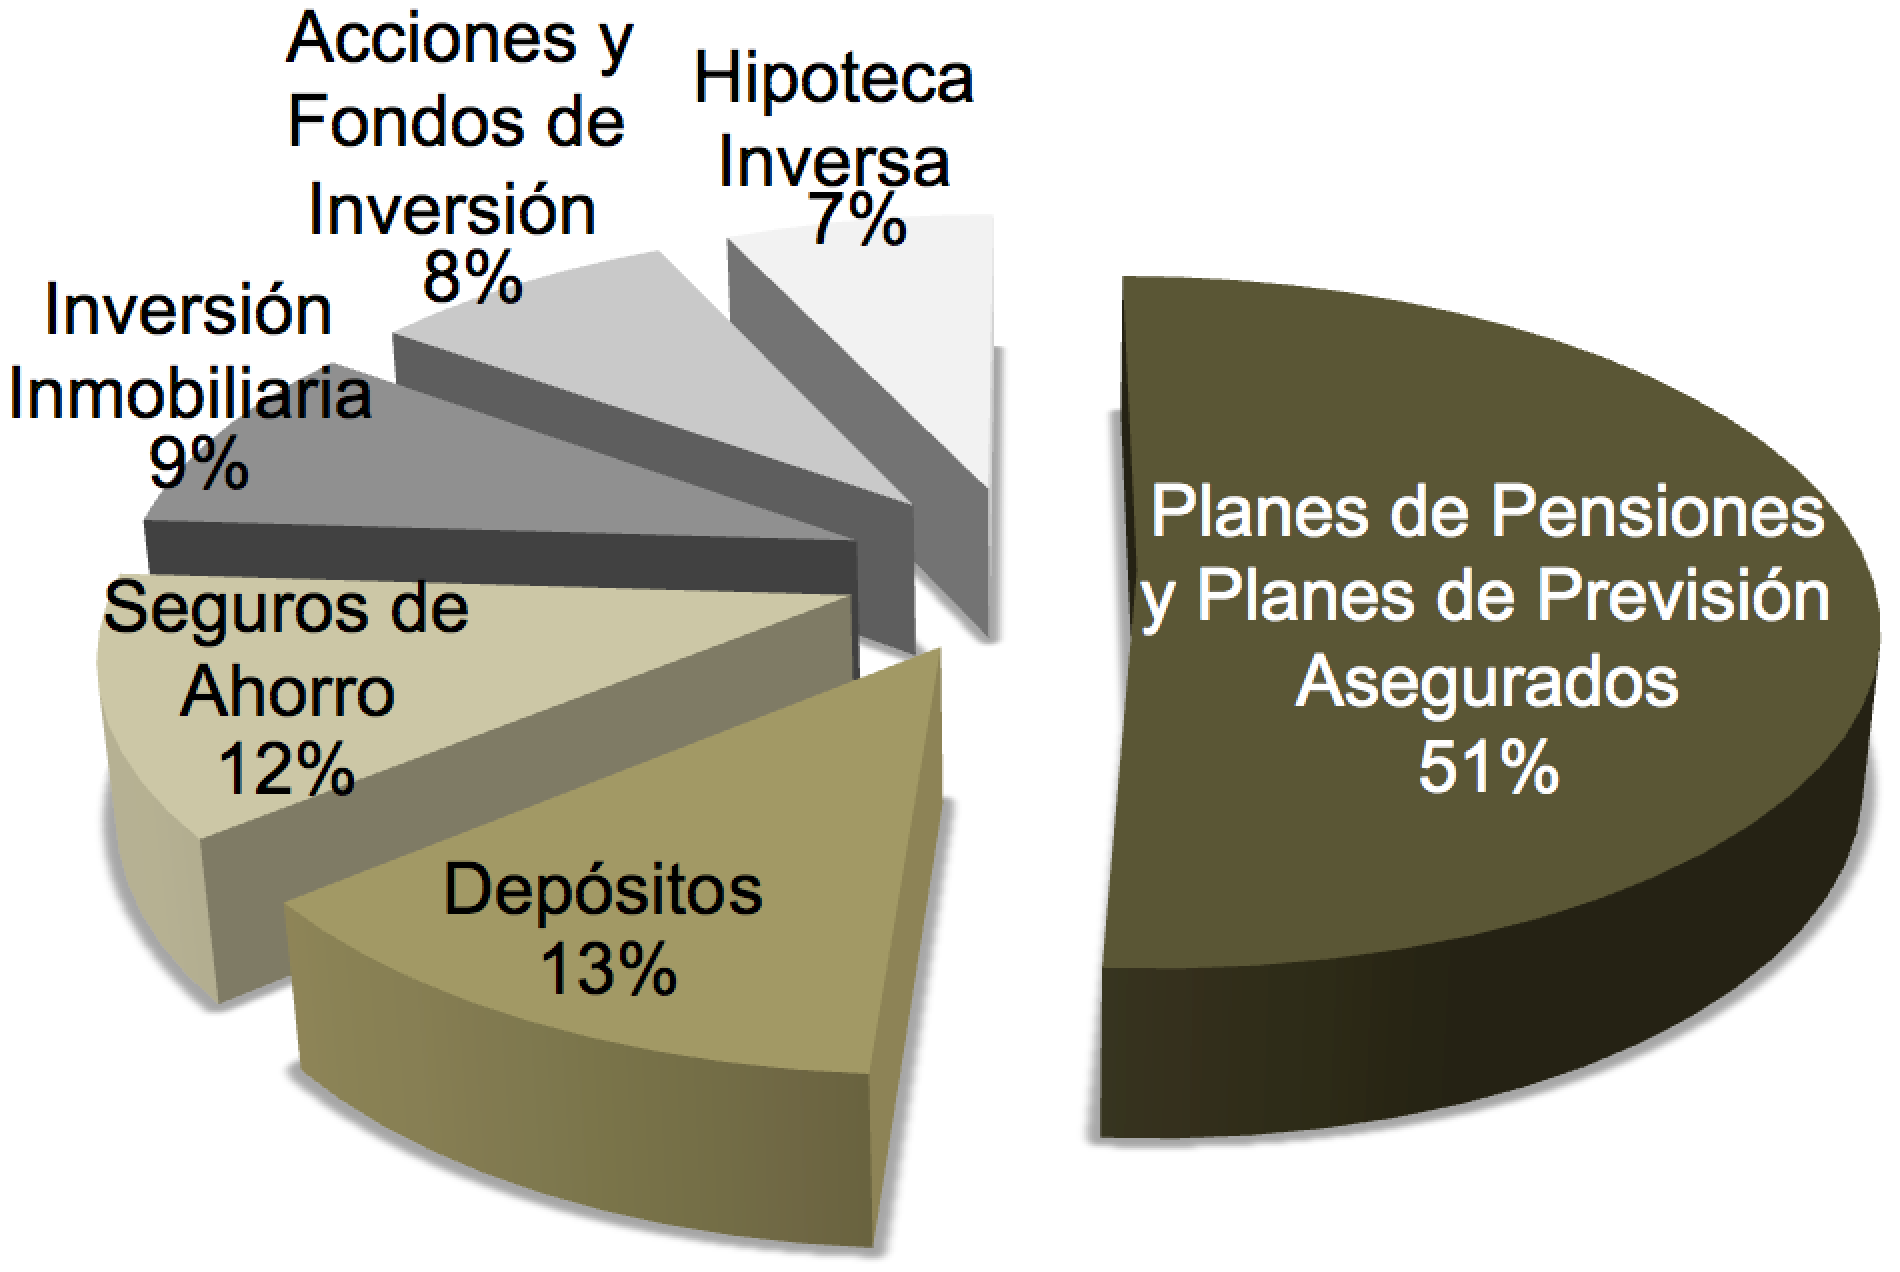
\includegraphics[width=\columnwidth]{ahorro2.png}}
						\caption{\small Instrumentos de ahorro m\'as preferidos. \textit{Fuente: Fundaci\'on y Vida}}
						\label{ahorro2}
					\end{figure}\vspace{-0.5cm}
					\begin{figure}[h]
						\fbox{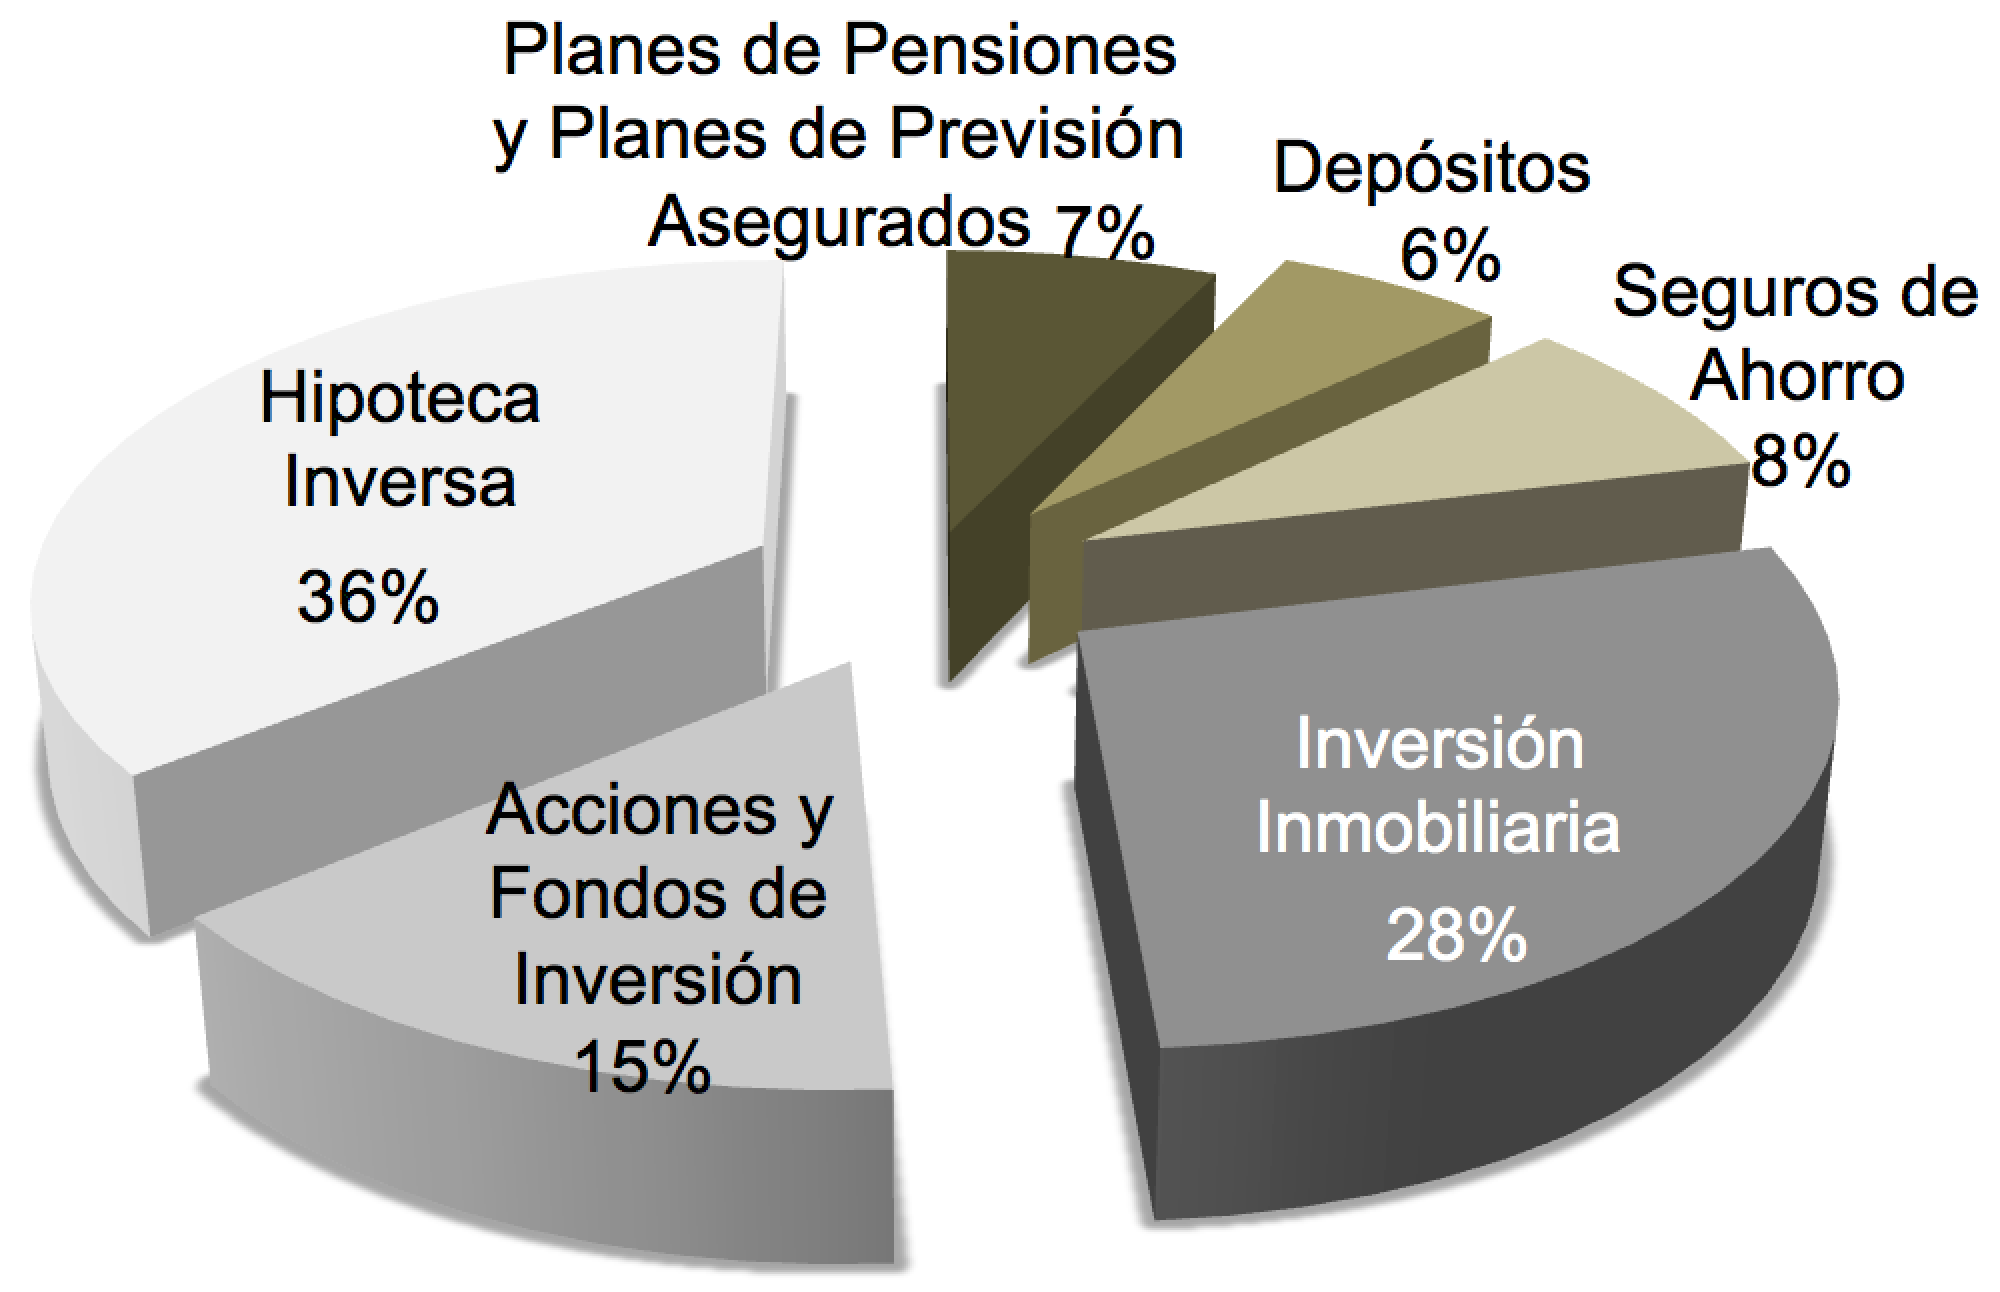
\includegraphics[width=\columnwidth]{ahorro1.png}}
						\caption{\small Instrumentos de ahorro menos preferidos.}
						\label{ahorro1}
					\end{figure}
			\end{columns}
		\end{block}
		
		\vspace{-1cm}
%%%%%%%%%%%%%%%%  PRINCIPALES RESULTADOS %%%%%%%%%%%%%%%%%%%%%%%%
		\begin{block}{La Hipoteca Inversa como Complemento a la Pensi\'on}\vspace{-0.8cm}
			\begin{multicols}{2}
				%\column{.48\columnwidth}
					\setlength{\parindent}{1.2em}	
					\setlength{\parskip}{1ex}
				\begin{itemize}
					%\item En la b\'usqueda de nuevas f\'ormulas de ahorro y previsi\'on, surge la figura de la hipoteca inversa.
					\item Poco conocida y  contratada en nuestro pa\'is, no tiene excesiva aceptaci\'on por diversos motivos:
						\begin{enumerate}
							\item[$\Rightarrow$] Caracter\'isticas del sector inmobiliario espa\~nol.
							\item[$\Rightarrow$] Dif\'icil de entender para los ancianos.
							\item[$\Rightarrow$] Implicaciones emocionales (apego a la vivienda).
							\item[$\Rightarrow$] Normalmente para inmuebles de alto valor.					
						\end{enumerate}
					\item A cambio de la propiedad de la vivienda, se recibe una especie de pensi\'on privada como alternativa o complemento a la pensi\'on p\'ublica.
					\item Al poner como garant\'ia esa vivienda de la que es titular, el prestatario recibe dinero mediante disposiciones peri\'odicas o en una sola entrega.
					\item Goza de beneficios fiscales y financieros.
					\end{itemize}
					\vspace{-1cm}		
					\begin{table}[h] 
						\begin{tabular}{|c|c|c|c|c|c|}
							\hline
							Edad & \multicolumn{4}{|c|}{\bfseries Valor tasaci\'on vivienda} & Duraci\'on\\ \cline{2-5}
							 & 100.000 & 200.000 & 300.000 & 400.000 & de la renta \\ \hline
							 \rowcolor[gray]{0.8}70 & 157,96 & 325,76 & 493,75 & 662,36 & 20 \\ \hline
							 75 & 218,49 & 447,06 & 676,30 & 905,78 & 17 \\ \hline
							 \rowcolor[gray]{0.8}80 & 306,36 & 623,22 & 941,39 & 1.259,29 & 14 \\ \hline
							 85 & 434,59 & 882,68 & 1.331,48 & 1.780,90 & 11 \\ \hline
							 \rowcolor[gray]{0.8}90 & 582,20 & 1.178,64 & 1.776,84 & 2.374,69 & 9 \\ \hline
							 %70 & 157,96 & 325,76 & 493,75 & 662,36 & 20 \\ \hline
						\end{tabular}
						\caption{Simulaciones de rentas mensuales temporales en funci\'on de la edad y del valor de la vivienda.}
						\label{renta}
					\end{table}
\vspace{-0.3cm}					
			\end{multicols}
			\vspace{-0.6cm}
			\noindent
			\begin{minipage}{.98\columnwidth}
				\begin{block}{Conclusiones}\vspace{-0.6cm}
					\begin{multicols}{2}
						\setlength{\parindent}{1.2em}	
						\setlength{\parskip}{1ex}
						\begin{itemize}
							\item Afrontamos un problema demogr\'afico de envejecimiento paulatino e incremento de las expectativas de vida.
							\item Se hace necesario minimizar el riesgo de longevidad mediante modelos de mortalidad fiables.
							\item Fundamental la planificaci\'on financiera: 
								\begin{enumerate}
									\item[$\Rightarrow$] \textbf{Estatal:} cambios en el sistema para garantizar las pensiones.
									\item[$\Rightarrow$] \textbf{Individual:} con productos alternativos que complementen la pensi\'on.
								\end{enumerate}
							\item La hipoteca inversa puede ser una opci\'on interesante que garantice liquidez para necesidades de consumo y m\'edicas o asistenciales durante la vejez.
						\end{itemize}
					\end{multicols}
					\vspace{-0.5cm}
				\end{block}
			\end{minipage}
		\end{block}
		\noindent
		
		\vspace{-0.45cm}
		
			\begin{block}{Extracto de la Bibliograf\'ia Destacada}\vspace{-0.4cm}
				\begin{itemize}
				\item[1.] P. Ehrlich: \textbf{The Population Bomb}, (1968) Ballantines Books 1era ed. 
				\item[2.] G. Tapinos: \textbf{Elementos de Demografía}, (1990) Espasa Universidad.
				\item[3.] H. \'Alvarez: \textbf{La Hipoteca Inversa: Una Alternativa en Tiempos de Crisis}, (2009) Lex Nova.
				%\item[3.] M. Ayuso y R. Holzmann: \textbf{Longevidad: Un Breve análisis Global y Actuarial}, \textit{Documento de Trabajo del Instituto BBVA de Pensiones} (2014).
				\item[4.] A. Villegas, V. K. Kaishev, P. Milosovich: \textbf{StMoMo: An R Package for Stochastic Mortality Modeling}, (2017).
				\item[5.] R. D. Lee y L. R. Carter: \textbf{Modeling and Forecasting U. S. Mortality}, Journal of the American Statistical Association, 87, 419, Septiembre (1992).
				\item[6.] C. Taffin: \textbf{La Hipoteca Inversa o Vitalicia}, Asociaci\'on Hipotecaria Espa\~nola (2004).
				%\item[7.] F.E. Wagner et al., \textbf{Electronic Structure and Properties of Hydrogen in Metals}, (1983), p. 581-595
				%\item[8.] [...]
				%\item[9.] [...]
				%\item[10.] [...]
				\end{itemize}\vspace{-0.3cm}
				\end{block}
			
	\end{columns}
\end{frame}
\end{document}
